% -*- mode: latex; -*- mustache tags:  
\documentclass[10pt,twoside,english]{_support/latex/sbabook/sbabook}
\let\wholebook=\relax

\usepackage{import}
\subimport{_support/latex/}{common.tex}

%=================================================================
% Debug packages for page layout and overfull lines
% Remove the showtrims document option before printing
\ifshowtrims
  \usepackage{showframe}
  \usepackage[color=magenta,width=5mm]{_support/latex/overcolored}
\fi


% =================================================================
\title{A PharoThings Tutorial}
\author{Allex Oliveira}
\series{Square Bracket tutorials}

\hypersetup{
  pdftitle = {A PharoThings Tutorial},
  pdfauthor = {Allex Oliveira},
  pdfkeywords = {IoT, Raspberry, PharoThings, Pharo}
}


% =================================================================
\begin{document}

% Title page and colophon on verso
\maketitle
\pagestyle{titlingpage}
\thispagestyle{titlingpage} % \pagestyle does not work on the first one…

\cleartoverso
{\small

  Copyright 2017 by Allex Oliveira.

  The contents of this book are protected under the Creative Commons
  Attribution-ShareAlike 3.0 Unported license.

  You are \textbf{free}:
  \begin{itemize}
  \item to \textbf{Share}: to copy, distribute and transmit the work,
  \item to \textbf{Remix}: to adapt the work,
  \end{itemize}

  Under the following conditions:
  \begin{description}
  \item[Attribution.] You must attribute the work in the manner specified by the
    author or licensor (but not in any way that suggests that they endorse you
    or your use of the work).
  \item[Share Alike.] If you alter, transform, or build upon this work, you may
    distribute the resulting work only under the same, similar or a compatible
    license.
  \end{description}

  For any reuse or distribution, you must make clear to others the
  license terms of this work. The best way to do this is with a link to
  this web page: \\
  \url{http://creativecommons.org/licenses/by-sa/3.0/}

  Any of the above conditions can be waived if you get permission from
  the copyright holder. Nothing in this license impairs or restricts the
  author's moral rights.

  \begin{center}
    
\includegraphics[width=0.2\textwidth]{_support/latex/sbabook/CreativeCommons-BY-SA.pdf}
  \end{center}

  Your fair dealing and other rights are in no way affected by the
  above. This is a human-readable summary of the Legal Code (the full
  license): \\
  \url{http://creativecommons.org/licenses/by-sa/3.0/legalcode}

  \vfill

  % Publication info would go here (publisher, ISBN, cover design…)
  Layout and typography based on the \textcode{sbabook} \LaTeX{} class by Damien
  Pollet.
}


\frontmatter
\pagestyle{plain}

\tableofcontents*
\clearpage\listoffigures

\mainmatter

\chapter{Lesson 1 – Turning LED on/off}
One of the classic analogies in electronics to “Hello World” is turn on a led or lamp. In this first lesson, we will learn how to connect correctly an LED to your Raspberry Pi and how to use PharoThings to control this led by turning it on and off.

Coding in Pharo is very simple, but it is very powerful and you can control all the GPIOs of your Raspberry Pi remotely.

If you did not yet see how to install the PharoThings on your Raspberry Pi and how to control it remotely, you can find the instructions in Chapter 1.
\section{What we need?}
In this lesson we will use a very simple setup.
\subsection{Components}
\begin{itemize}
\item 1 Raspberry Pi connected to your network (wired or wireless)
\item 1 Breadboard
\item 1 LED
\item 1 Resistor (330ohms)
\item Jumper wires
\end{itemize}
\section{Experimental theory}
Before constructing any circuit, you must know the parameters of the components in the circuit, such as their operating voltage, operating circuit, etc.
\subsection{The LED}
To turn on the LED, we need to send the correct voltage and current to it. The voltage and current can’t be too high, otherwise, the led will burn, or in some cases, damage the Raspberry.

Typically, the forward voltage of an LED is between 1.8 and 3.3 volts. It varies by the color of the LED. A red LED typically drops 1.8 volts, but voltage drop normally rises as the light frequency increases, so a blue LED may drop from 3 to 3.3 volts{[}1{]}.

Most 3mm and 5mm LEDs will operate close to their peak brightness at a drive current of 20 mA. This is a conservative current: it doesn’t exceed most ratings (your specs may vary, or you may not have any specs–in this case, 20 mA is a good default guess {[}2{]})

In this experiment, the operating voltage of the LED is between 1.5V and 2.0V and the operating current is between 10mA and 20mA.
\subsection{The Resistor}
We must always use resistors to connect LEDs up to the GPIO pins of the Raspberry Pi to limit the voltage and current between the LED and the Raspberry to a safe value.

A small change in voltage can produce a huge change in current (see more: LED Current vs. Voltage {[}2{]})

In this experiment, we will use a 330ohm resistor. To identify the correct resistor, follow one of the following color sequences, depending on the number of bands {[}3{]}:

\begin{itemize}
\item If there are four colour bands, they will be Orange, Orange, Brown, and then Gold;
\item If there are five bands, then the colours will be Orange, Orange, Black, Black, Brown.
\end{itemize}

It does not matter which way round you connect the resistors (in this experiment). Current flows in both ways through them. This means that you can connect the resistor at the positive pole or the negative pole of the LED, as well as starting with the first or last color, as shown in the Picture \ref{Ledpolarity}.

But the LEDs will only work if the power is supplied correctly (if the polarity is correct). You will not burn the LEDs if they connect the wrong way – they just will not turn on.


\begin{figure}

\begin{center}
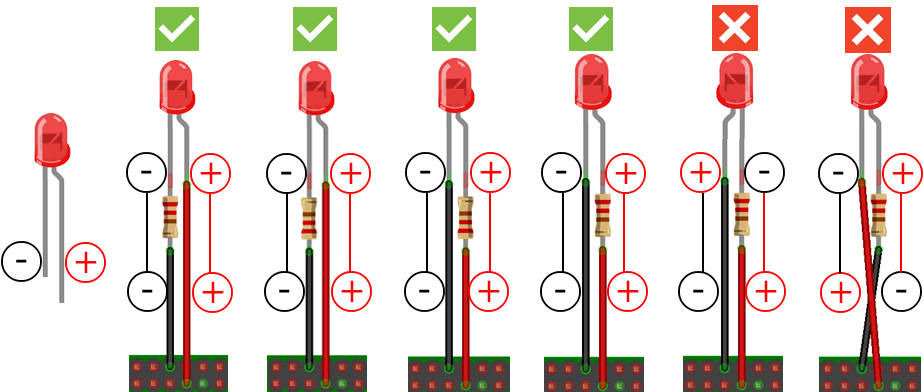
\includegraphics[width=0.6\textwidth]{/Users/allexoliveira/PharoThingsBook/Booklet-APharoThingTutorial/_result/pdf/Chapters/Chap2LED/figures/pharothings-led-polarity-resistors.png}\caption{Led polarity and resistors.\label{Ledpolarity}}\end{center}
\end{figure}

\subsection{The Breadboard}
A breadboard is used to build prototyping of electronics. With a breadboard, it is not necessary to use solder, this way you can reuse the board. This makes it easy to use to create temporary prototypes and experiment with circuit design.

The holes in the breadboard are connected following a pattern, as shown in the Picture \ref{Breadboard}.

\begin{itemize}
\item The red (+) and blue (-) rail are connected horizontally;
\item The holes in the middle are connected vertically.
\end{itemize}


\begin{figure}

\begin{center}
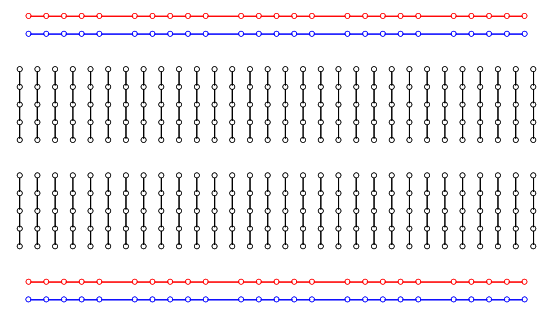
\includegraphics[width=0.6\textwidth]{/Users/allexoliveira/PharoThingsBook/Booklet-APharoThingTutorial/_result/pdf/Chapters/Chap2LED/figures/pharothings-breadboard.png}\caption{Breadboard scheme.\label{Breadboard}}\end{center}
\end{figure}

\section{Experimental procedure}
Now we will build the circuit. This circuit consists of an LED that lights up when power is applied, a resistor to limit current and a power supply (the Rasp).

\begin{itemize}
\item Connect the Ground PIN from Raspberry in the breadboard blue rail (-). Raspeberry Pi models with 40 pins has 8 GPIO ground pins. You can connect with anyone. In this experiment we will use the PIN6 (Ground);
\item Then connect the resistor from the blue rail on the breadboard (-) to a column on the breadboard, as shown in the Picture \ref{physicalLed};
\item Now push the LED legs into the breadboard, with the long leg (with the kink) on the right;
\item And insert a jumper wire connecting the rigth column and the PIN7 (GPIO7).
\end{itemize}

The Figure \ref{physicalLed} shows how the electric connection is made:


\begin{figure}

\begin{center}
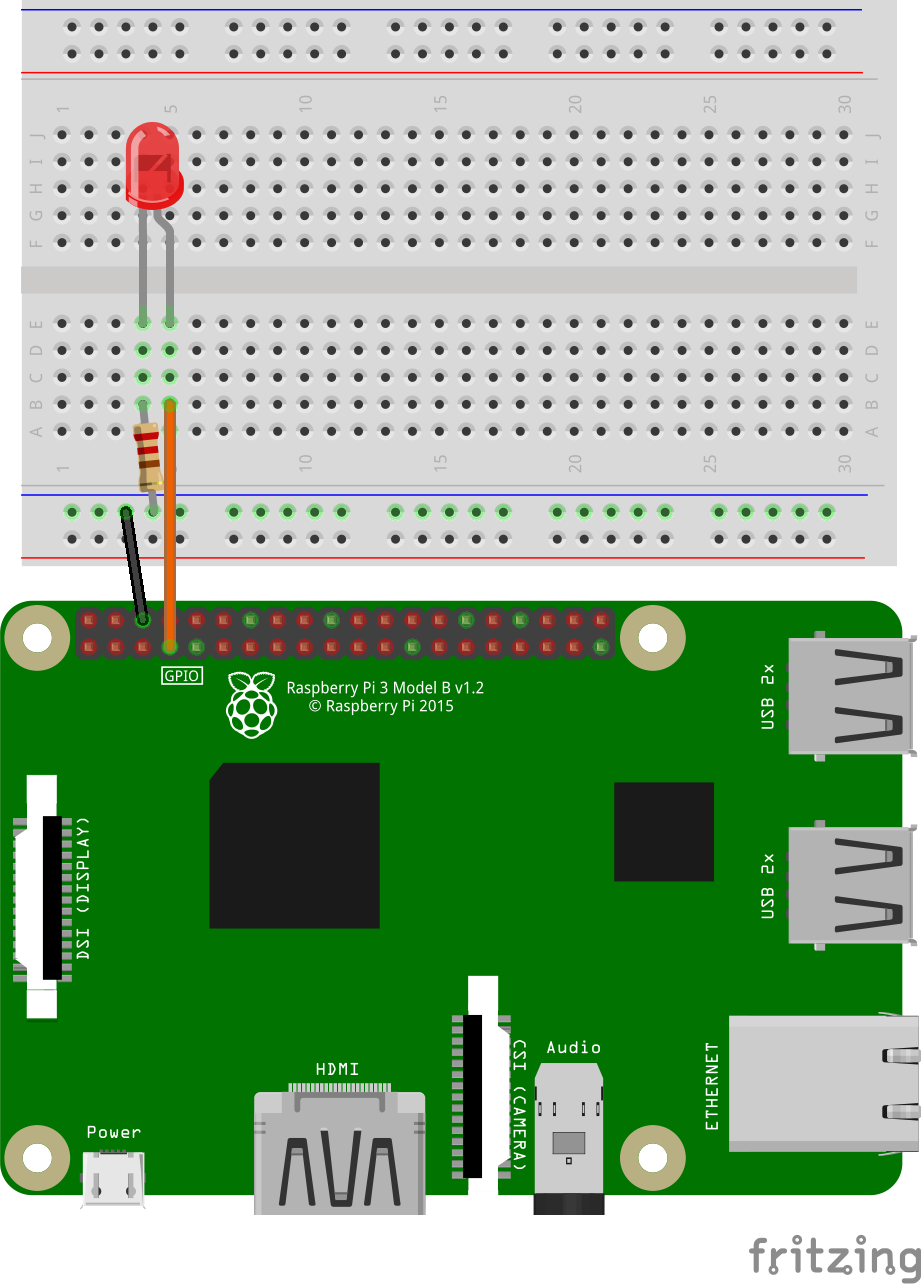
\includegraphics[width=0.6\textwidth]{/Users/allexoliveira/PharoThingsBook/Booklet-APharoThingTutorial/_result/pdf/Chapters/Chap2LED/figures/pharothings-raspberry-led-resistor-lesson-01.png}\caption{Physical connection LED.\label{physicalLed}}\end{center}
\end{figure}

\section{Experimental code}


Now, we can write some code in Pharo to control the GPIOs using PharoThings and turn the LED on. We have 2 options to do this:

\begin{itemize}
\item Write the code locally on the Raspberry;
\item Use TelePharo to connect from your computer into the Raspberry and do all the work remotely.
\end{itemize}

In this experiment, we will use the second option: connect and do all the work remotely. 

If you didn’t see how to install the PharoThings on your Raspberry Pi and how to control it remotely, take a look in the Chapter 1: Installations.
\subsection{Connecting remotely}
Through your local Pharo image, let's connect in the Pharo image running on Raspberry, enable the auto-refresh feature of the inspector and open the inspector. Run this code in your local playground:

\begin{displaycode}{plain}
remotePharo := TlpRemoteIDE connectTo: (TCPAddress ip: #[193 51 236 167] port: 40423)
GTInspector enableStepRefresh
remoteBoard := remotePharo evaluate: [ RpiBoard3B current].
remoteBoard inspect.
\end{displaycode}

In your inspect window (Inspector on a PotRemoteBoard) you can see a scheme of pins similar to the Raspberry Pi docs. But here it is a live tool which represents the current pins state.


\begin{figure}

\begin{center}
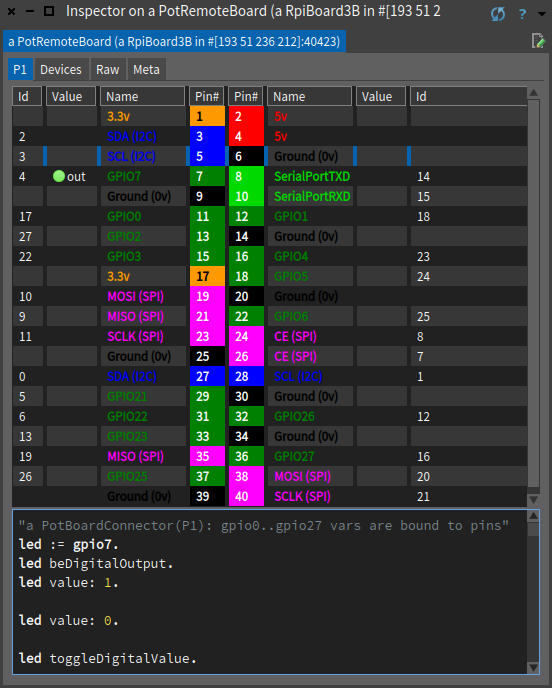
\includegraphics[width=0.6\textwidth]{/Users/allexoliveira/PharoThingsBook/Booklet-APharoThingTutorial/_result/pdf/Chapters/Chap2LED/figures/pharothings-inspector-remote-board-raspberry.png}\caption{Remote Board Inspector.\label{remoteBoard}}\end{center}
\end{figure}


Digital pins are shown with green/red icons which represent high/low (1/0) values. In case of output pins you are able to click on the icon to toggle the value.

To control the led we first introduce the named variable \#led which we assigned to GPIO7 pin instance:

\begin{displaycode}{plain}
led := gpio7.
\end{displaycode}

Then we configure the pin to be in digital output mode and set the value:

\begin{displaycode}{plain}
led beDigitalOutput.
led value: 1.
\end{displaycode}

It turnes the led on.

You can notice that gpio variables are not just numbers/ids. PharoThings models boards with first class pins. They are real objects with behaviour. For example you can ask pin to toggle a value:

\begin{displaycode}{plain}
led toggleDigitalValue.
\end{displaycode}

Or ask a pin for current value if you want to check it:

\begin{displaycode}{plain}
led value.
\end{displaycode}
\section{What did we learn?}
With PharoThings you can remotely control all the GPIOs in your running board!

You can:

\begin{itemize}
\item Interact remotely with pins and boards;
\item See the current pins state in real time;
\item Run the code dynamically.
\item Easy, powerful.
\end{itemize}
\section{In the next lesson}
Let’s use what we learned in this lesson and write a simple code to blink the LED.


% lulu requires an empty page at the end. That's why I'm using
% \backmatter here.
\backmatter

% Index would go here

\end{document}
